\documentclass[10pt]{article}
\usepackage[polish]{babel}
\usepackage[utf8]{inputenc}
\usepackage[T1]{fontenc}
\usepackage{amsmath}
\usepackage{amsfonts}
\usepackage{amssymb}
\usepackage[version=4]{mhchem}
\usepackage{stmaryrd}
\usepackage{graphicx}
\usepackage[export]{adjustbox}
\graphicspath{ {./images/} }

\begin{document}
\begin{enumerate}
  \item Liczba 999...9 jest zapisana za pomocą 999 dziewiątek. Ile wynosi suma cyfr kwadratu tej liczby? Podać wynik w postaci konkretnej liczby, zapisanej za pomocą kolejnych cyfr, nie zaś iloczynu, kwadratu itp.
  \item W turnieju szachowym w grupie A było \(n\) zawodników, a w grupie B 2n zawodników. W każdej grupie każdy grał z każdym. W grupie B rozegrano \(k(k \in N)\) razy więcej meczów niż w grupie A. Wyznacz wszystkie możliwe pary ( \(n, k\) ).
  \item Dane są dwa kwadraty, jeden przy drugim, o bokach \(a\) i \(b\). Wyznacz stosunek pól: zamalowanej części dużego kwadratu i tegoż kwadratu.\\
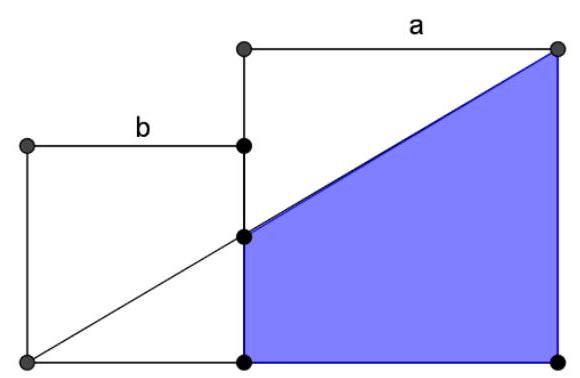
\includegraphics[max width=\textwidth, center]{2024_11_21_cc19a29450c490975967g-1}
\end{enumerate}

\end{document}